% What stl2bem does, at a glance: an STL in, the sound pressure on its surface out.
% Larger type than the other figures: this one is shown at the top of the README at about 880 px.
% Shared figure style for stl2bem (compile with XeLaTeX; build.sh).
% Two hues only: navy for stl2bem and its results, gray for references and the original code; variants inside a hue
% differ by marker, line style and weight. Raster pieces come from rasters.py with the same color stops.
\documentclass[border=2pt]{standalone}
\usepackage{fontspec}
\usepackage{tikz}
\usepackage{pgfplots}
\usepgfplotslibrary{groupplots}
\usetikzlibrary{arrows.meta,positioning,calc}
\pgfplotsset{compat=1.18}
\setmainfont{texgyreheros}[Extension=.otf, UprightFont=*-regular, BoldFont=*-bold, ItalicFont=*-italic,
  BoldItalicFont=*-bolditalic, Scale=0.95]

\newcommand{\fs}{\fontsize{8pt}{9.6pt}\selectfont}
\newcommand{\fss}{\fontsize{7pt}{8.4pt}\selectfont}
\newcommand{\fsl}{\fontsize{9pt}{10.8pt}\selectfont}
\newcommand{\panel}[1]{\textbf{(#1)}}
% symbols in the text font (no serif maths in the figures)
\newcommand{\vp}{\textit{p}}
\newcommand{\ka}{\textit{ka}}
\newcommand{\minus}{\textendash}
\newcommand{\pow}[2]{#1\textsuperscript{\minus#2}}

\definecolor{cNavy}{HTML}{1F4E79}
\definecolor{cNavyM}{HTML}{7FA0C2}
\definecolor{cNavyL}{HTML}{C9D7E6}
\definecolor{cGrey}{HTML}{6B7280}
\definecolor{cGreyL}{HTML}{A7ADB6}
\definecolor{cInk}{HTML}{1F2933}
\definecolor{cMuted}{HTML}{7B8794}
\definecolor{cGrid}{HTML}{E9EBEE}
\definecolor{cBody}{HTML}{3E4752}

\pgfplotsset{
  colormap={div}{rgb255=(47,54,64) rgb255=(141,149,160) rgb255=(255,255,255) rgb255=(94,134,174) rgb255=(18,49,79)},
  colormap={seq}{rgb255=(255,255,255) rgb255=(201,215,230) rgb255=(127,160,194) rgb255=(31,78,121) rgb255=(15,42,68)},
  every axis/.append style={
    font=\fs, line width=0.5pt,
    tick label style={font=\fss, text=black, /pgf/number format/assume math mode=true},
    label style={font=\fs, text=black}, title style={font=\fsl, text=black},
    tick style={cMuted, line width=0.5pt}, major tick length=2pt,
    axis line style={cMuted, line width=0.6pt},
    legend style={font=\fss, draw=none, fill=none, legend cell align=left, inner sep=1pt},
    grid style={cGrid, line width=0.4pt},
  },
  mapaxis/.style={axis equal image, axis on top, ticks=none, enlargelimits=false, scale only axis,
    axis line style={cInk, line width=0.6pt}},
  cbar/.style={colorbar style={width=2.2mm, font=\fss, axis line style={cMuted}, tick style={cMuted},
    ytick style={cMuted}, yticklabel style={font=\fss}}},
}

\setmonofont{DejaVu Sans Mono}[Scale=0.88]
\renewcommand{\fss}{\fontsize{10pt}{12pt}\selectfont}
\renewcommand{\fsl}{\fontsize{13pt}{15.6pt}\selectfont}
\begin{document}
\begin{tikzpicture}[text=black, >=Stealth]
  \node[inner sep=0] (in) at (0,0) {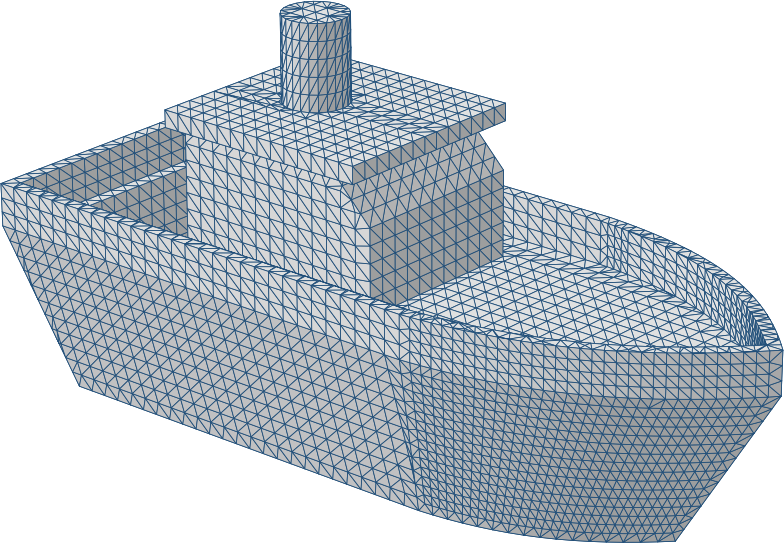
\includegraphics[height=3.2cm]{raster/stl_boat_mesh.png}};
  \node[inner sep=0, anchor=west] (out) at ([xshift=4.4cm]in.east) {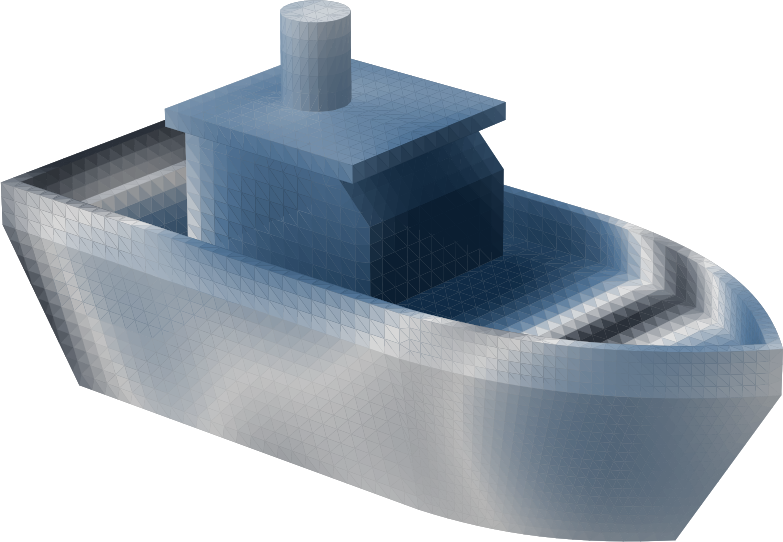
\includegraphics[height=3.2cm]{raster/stl_boat_pressure.png}};
  \draw[->, cNavy, line width=1.6pt] ([xshift=0.5cm]in.east) -- ([xshift=-0.5cm]out.west)
    node[midway, above=3pt, text=black, font=\fsl\bfseries] {stl2bem}
    node[midway, below=4pt, text=black, font=\fss] {boundary element method};
  \node[anchor=north, font=\fsl, align=center] at ([yshift=-0.3cm]in.south)
    {\texttt{body.stl}\\[2pt]{\fss triangle mesh from CAD}};
  \node[anchor=north, font=\fsl, align=center] at ([yshift=-0.3cm]out.south)
    {sound pressure\\[2pt]{\fss on the surface}};
\end{tikzpicture}
\end{document}
